
\section{Research Contributions}


blah


\section{Implications for Urban Planning}

blah


\section{Future Research}




\subsection{Improving Theory About Urban Dynamics And Activity Behaviour}


% overview
Neighbourhoods are the stage for daily life. Individuals' neighbourhood contexts can impact a number of social outcomes; from daily travel behaviour and activity participation, to longer-term effects on employment, income, health, and well-being \cite{sampson_assessing_2002,ewing_travel_2010,lucas_transport_2012,bastiaanssen_does_2020}. These are often called \textit{neighbourhood effects}. However, environmental contexts change over longer period of time, both in terms of their built environments (e.g. due to land use intensification, transit (dis)investments) and social attributes (e.g. socioeconomic decline, gentrification) \cite{van_ham_understanding_2013,wegener_land-use_2004}. Therefore, one's environmental exposures are not static nor consistent over time, they are sensitive to these \textit{neighbourhood dynamics}. 

Scale, nexus of the individual and the global. 
These longer-term changes are also a product of individual preferences and decisions in aggregate. i.e. neighbourhoods effect individual outcomes, and individuals shape neighbourhoods.


% research goal
The objective of this paper is to present a conceptual framework that synthesizes theories of travel behaviour, neighbourhood effects, and neighbourhood dynamics into a symbiotic whole, one that conveys how neighbourhood effects and neighbourhood dynamics are part of a multi-scalar system of cyclical feedback effects. This is based on combining several related strands of research: 1) research examining environmental effects on daily travel and activity behaviour \cite{hanson_determinants_1982,ewing_travel_2010}; 2) how one's location and preferences impacts resource acquisitions such as housing choices or purchasing a car \cite{lee_neighborhood_1994,klein_millennials_2017}; 3) the effects of prolonged exposures to environments on long-term social outcomes like employment, income, and education \cite{sampson_assessing_2002,chetty_effects_2016}, which are often propagated via feedback effects \cite{wilson_truly_2012,lucas_transport_2012}; and 4) how individual actions, in aggregate, can cause the physical and social characteristics of neighbourhoods to change over time via transport investments, land use change, and residential mobility decisions \cite{wegener_land-use_2004,wilson_truly_2012,van_ham_understanding_2013}. 



In this section, we present a integrated conceptual framework to bring together the aforementioned conceptualizations of how geographic contexts effect individual outcomes, with how these geographic contexts can change over time. 

Why is this important? Implications for research , while controlling , 

human systems, urban systems, are complex - finding order within this complexity ...

The overall framework is shown in Figure 2. This is divided into individual attributes and outcomes, geographic (i.e. neighbourhood) contexts, and global factors. The QQQ lines pertain to effects on individual choices and outcomes, while the QQQ lines pertain to aggregate effects of individuals on neighbourhood and regional characteristics.

Sampson 2019/2012 - cogs micro/macro effects

feedback - lucas

UGCP - Kwan


% social outcomes, such as examining the impacts of changing environmental contexts on travel behaviour \cite{caoChangesNeighborhoodCharacteristics2007},


\begin{figure}[H]
	\caption{Combined conceptualization}
	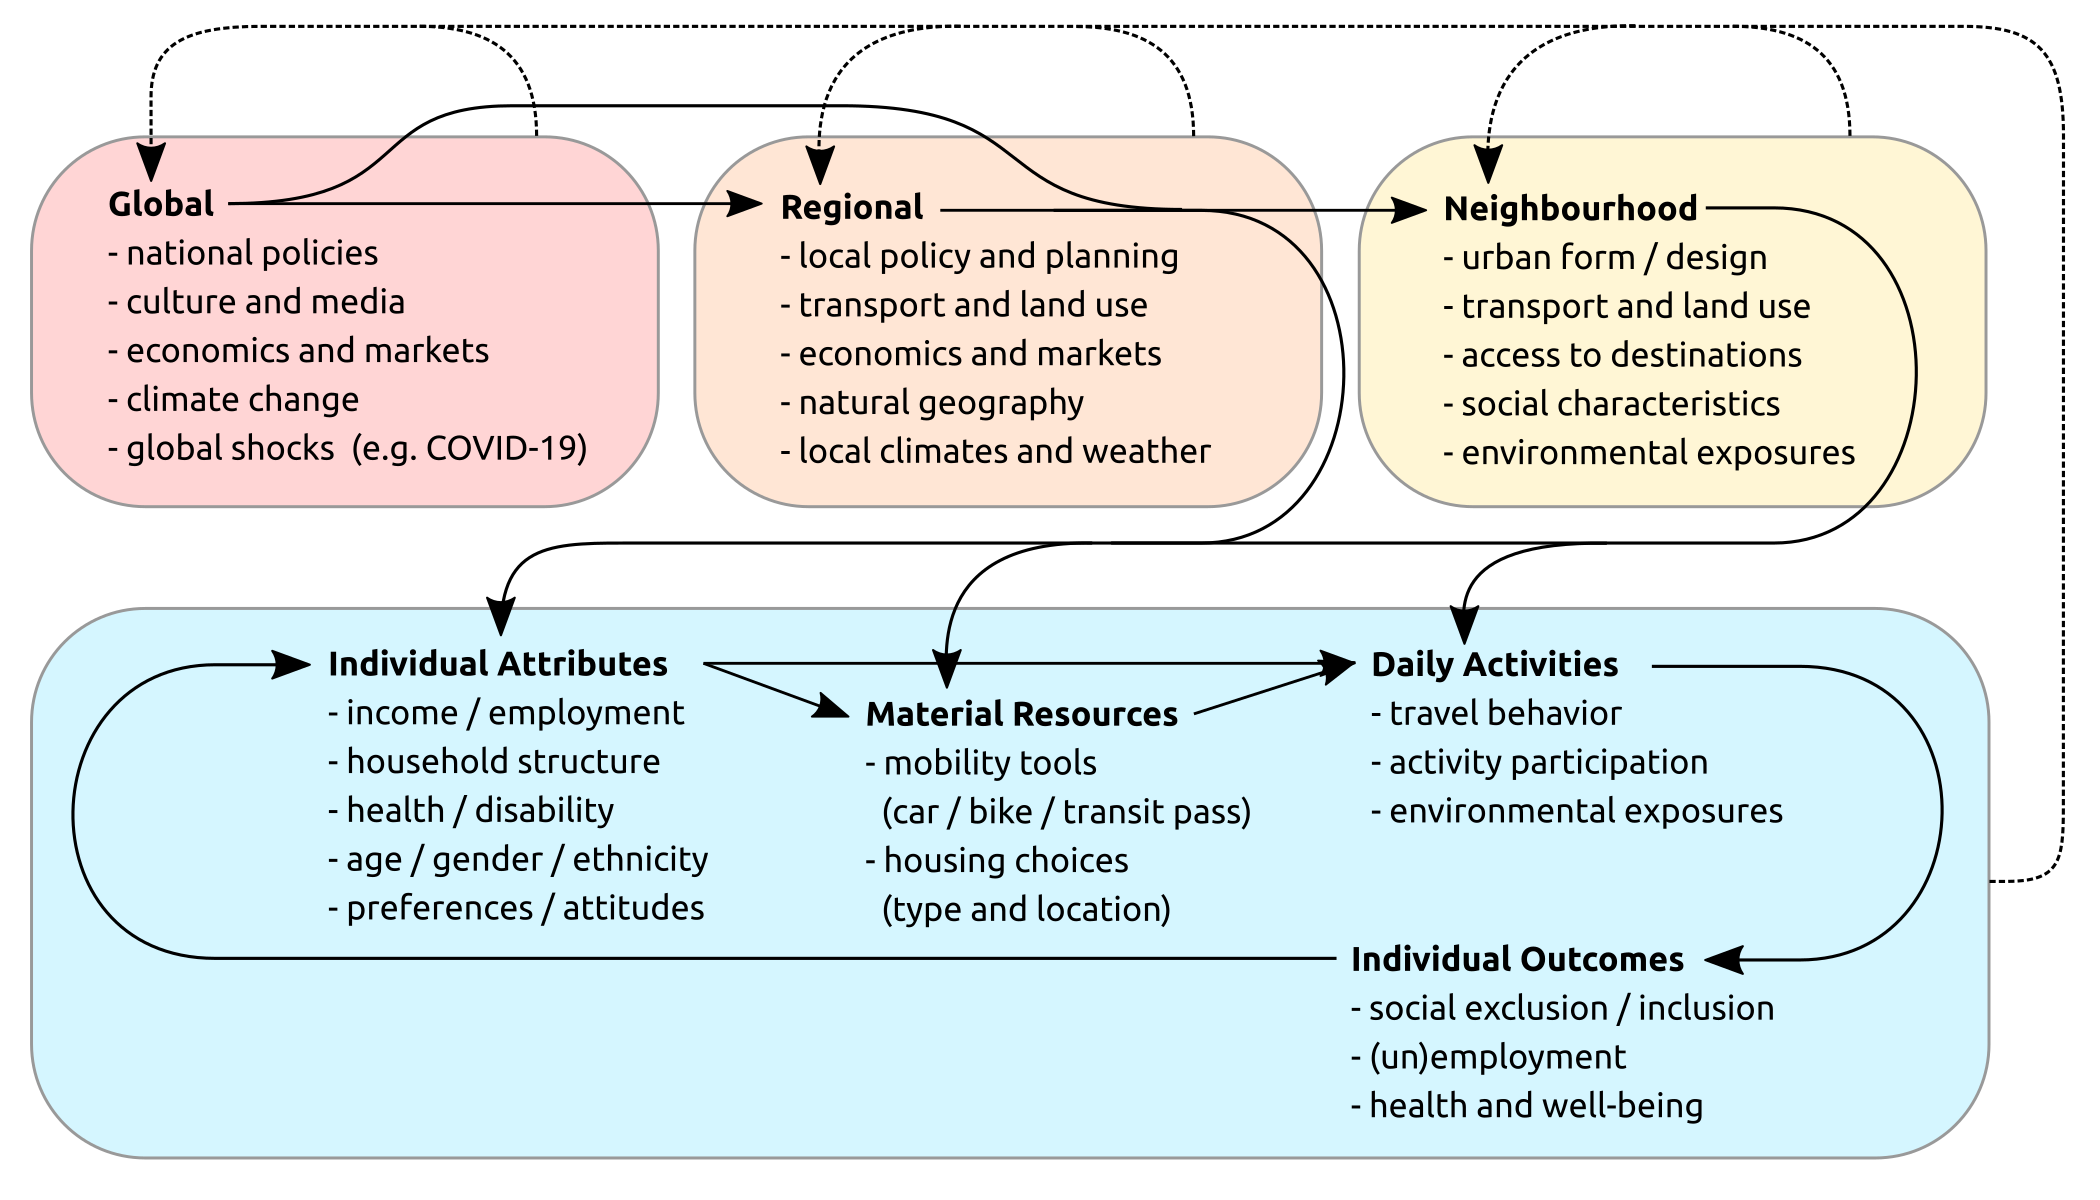
\includegraphics[width=7in]{figures/my_idea.png}
	\centering
\end{figure}




\subsection{Transit-Induced Displacement In Canada}

Beep, expanding upon prev chapter

% transportation urban form income mobility - need data on auto ownership



\subsection{Transit Accessibility, Urban Form, and Income Mobility}

Ample research has shown that compact urban forms and greater levels of transit accessibility promote more environmentally friendly outcomes and healthier lifestyles \cite{ewing_compactness_2015,ewing_travel_2010,cervero_travel_1997}. There are also theoretical arguments that accessibility is a social good, as it enables activity participation \cite{martens_transport_2016,pereira_distributive_2017}.
But what about long-term benefits? Can such built environments also lead to social mobility and poverty reduction? Research has noted how neighbourhood socio-economic effects impact individual social mobility \cite{chetty_effects_2016}, yet research on how urban form, and in particular transit accessibility has on long term social outcomes is sparse \cite{ewing_does_2016,fransen_relationship_2019}.
(I will need to do some more research to see what else has been done with the MOT study and the PSID in the USA, as I think there are a few papers that look at urban form and car ownership on social mobility \cite{smart_disentangling_2020}. There is nothing that I'm aware of in Canada however. There's also quite a few studies that look at the unemployment-accessibility relationship, but few are longitudinal and individual level).

This chapter will use the same data is the previous one, but will attempt to uncover whether low-income residents exposed to more compact urban forms and better levels of transit accessibility have relatively greater income mobility over time relative to areas of worse accessibility, while controlling for other demographic and stage-of-life effects, as well as residential mobility and exposure to different urban forms. In particular, the Longitudinal Administrative Data/Databank/Database (LAD) will be the primary dataset for this paper, as it includes basic demographics (age, gender, marital status) and household structure (info about family members), as well as sources of income included in tax records. One limitation of this data, however, is it does not include information on car ownership, despite it being shown to be related to earnings in the long-term \cite{smart_disentangling_2020}.

For methods, my current thinking is to model change in income, $\Delta I_i$ via a combination of level of accessibility, $A$, urban form, $U$, and controlling for demographic and households characteristics, $X$, and neighbourhood socio-economic variables, $N$.

\[
\Delta I_i = c + \alpha A_i + \mu U_i + \nu N_i + \beta X_i + \epsilon_i
\]

$\Delta I_i$ will be considered first as an absolute value pertaining to after-tax income, scaled to the most recent year's currency value. I will then convert income to measures of equivalent household income, which would then allow for generating measures of poverty based on the LIM methodology\footnote{divide income by the square root of households size, then compare with the distribution of all households. Those less than 50\% of the median are deemed to be under the poverty line}. 
$N$, $A$, and $U$ will be based on one's average if they have moved to over the period of study. It will also be good to add a variable indicating residential mobility. The model will likely require incorporating multilevel effects, for both individual and neighbourhood scales. Spatial effects will be tested at the neighbourhood level. Another modelling option that I'll try to specify is more of an experimental design, where instead of a mean level of accessibility, $A$ and $U$ will be categorical variables pertaining to an increase, decrease, and no-change in accessibility for a specific time period, $t$, caused by a residential mobility event or opening of a new transit line. This strategy could be differentiated or combined for multiple intervention periods.

Overall, the hope is that the sign and significance of the coefficients $\alpha$ and $\mu$ will offer evidence into whether, and to what extent, living in different types of built environments can have on income mobility and poverty reduction. Results will thus provide knowledge about whether and how the built environment (e.g. accessibility and urban form) can be a catalyst for neighbourhood SES change, and how different urban transport planning and design strategies can alleviate poverty.



% future transit accessibility

\subsection{Transportation Forecasting With Urban Dynamics}

Future forecasting with urban dynamics.

Urban futures are rife with uncertainty. Yet when planners and researchers assess the distributions of transit accessibility benefits across different socio-economic groups, they are typically based on current distributions. However, it is clear that the demographic patterns of cities change over time, as recently evidenced by socio-spatial polarization, gentrification, and suburbanization of poverty. As such, transport planners should be mindful of potential socio-economic changes when they examine current and future distributions of transport accessibility, as they can directly relate to social (in)equity and transport-related social exclusion. Accordingly, future research should explore how the distributions of transit accessibility relative to socio-econmoic status can vary substantially depending on different future socio-economic trajectories. Examples of differing trajectories include gentrification versus affordable near transit and polarization versus evenness. 

This could be explored through a theoretical discussion and conceptual examples; simulating data based on current (2016) population, employment, and transit travel time data as base, and apply ranges of outcomes based on the above dimensions. 
SES will be considered as counts of readily available census data such as low-income households by zone, recent immigrants, and other low-SES population groups, likely defined based on my findings in the previous papers. The study area(s) for this part are currently open. I currently have transit travel time data for eight of the largest urban regions in Canada, so any one or more of them could be studied. Simulations will make use of Markov chain Monte Carlo methods, based on stochastic transition matrices generated by parameters relating to polarization-evenness, gentrification-affordability, homophily, and spatial focus of residential mobility. 

Third, I will explore these issues using a regional travel demand model of the Toronto region, specifically by tweaking it's residential mobility sub-model. Access to this model and information of what parameters can be adjusted will require further discussion with the Travel Modelling Group\footnote{\url{https://tmg.utoronto.ca/}} at the Civil Engineering department. The benefit of this approach is that it is a fully integrated model. In other words, it will provide differing outputs for population, land-use, and travel times depending on variation in input parameters. This will allow for computing accessibility measures for multiple scenarios, rather than comparing multiple socio-economic distributions with a single accessibility distribution.

My current expectation is that results will likely indicate that compact urban forms, focused on affordable housing near transit will reap the greatest benefits in terms of social equity and social inclusion.




\subsection{Communication}



